\subsection{Показатель Ляпунова}

Рассмотрим гладкое отображение $u_{t+1} = f(u_t)$. Пусть имеются две траектории этой системы $\{u_i\}_{i=1}^{\infty}$ и $\{u'_i\}_{i=1}^{\infty}$, порожденные достаточно близкими начальными точками $u_0$, $u'_0$. Чтобы определить расстояние между этими двумя орбитами, для начала определим расстояние между точками $u_1$ и $u'_1$:
$$
        u_1-u'_1 = f(u_0)-f(u'_0) = f'(u_0)(u_0-u'_0)+o(|u_0-u'_0|).
$$
Если $|f'(u_0)| < 1$, то в линейном приближении расстояние между двумя точками $u_1$ и $u'_1$ будет меньше, чем расстояние между начальными точками орбит $u_0$ и $u'_0$. Тогда если $|f'(u_{k-1})| < 1$ ($>1$), то расстояние между точками будет уменьшаться (увеличиваться). Так как производная в точке $u_t$ функции $f(u)$ как больше, так и меньше единицы в зависимости от значения $t$, то есстественно считать за меру близости некоторую среднюю величину, высчитываемую по всем возможным значениям $t$. Такая величина называется числом или показателем Ляпупова. \cite[стр.~93]{bratus10}

\begin{definition}
        Пусть $f:\R\rightarrow\R$~--- гладкое отображение. Числом Ляпунова траектории $\{u_i\}_{i=1}^{\infty}$ называется величина
        $$
                l(u_0) = \lim\limits_{n \to \infty}\left( |f'(u_0)| \cdot |f'(u_1)| \cdot \ldots \cdot |f'(u_n)| \right)^{\frac{1}{n}}.
        $$
        \cite[стр.~94]{bratus10}
\end{definition}
            
\begin{definition}
        Показателем Ляпунова траектории $\{u_i\}_{i=1}^{\infty}$ называется величина
        $$
                h(u_0) = \ln(l(u_0)) = \lim\limits_{n \to \infty} \frac{\ln|f'(u_0)| + \ln|f'(u_1)| + \ldots + \ln|f'(u_n)|}{n},
        $$
        если этот предел существует. \cite[стр.~94]{bratus10}
\end{definition}
            
\begin{figure}[h]
        \centering
        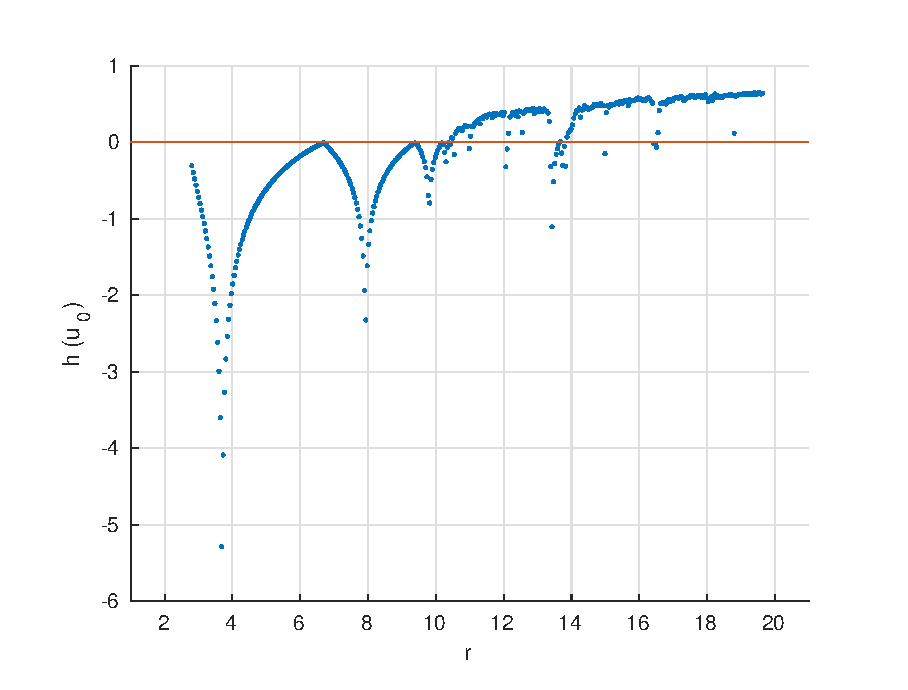
\includegraphics[width=0.6\linewidth]{img/one_step_lyapunov.eps}
        \caption{Показатель Ляпунова при начальном приближении приближении $u_0 = 4$.}
        \label{img:one_step_lyapunov}
\end{figure}